\section{Risultati della sperimentazione}
Si presentano ora i risultati quantitativi della sperimentazione effettuata sui
cinque pannelli scelti. Come anticipato, 
avendo un numero 
ridotto di sample a disposizione, si è scelto di estrarre da ogni pannello 100
sample 
da usare come query per il calcolo degli $\SMEM$, riducendo il numero di
sample a 4.908. 
\subsection{Costruzione delle strutture e calcolo degli SMEM}
Viste le dimensioni di tali pannelli, si ritiene necessario studiare, dal punto
di vista del tempo macchina e dei picchi di memoria necessaria, le varie fasi
della sperimentazione, ovvero:
\begin{itemize}
  \item la fase di preprocessing, necessaria per la preparazione dei
  vari input della $\RLPBWT$, comprendente: 
  \begin{itemize}
    \item la conversione dei file in formato VCF nei file in formato MaCS\footnote{\url{https://github.com/gchen98/macs}}, usato 
    come formato di input nella $\RLPBWT$
    \item l'estrazione del pannello delle query e la creazione del nuovo
    pannello di aplotipi
    \item la produzione dell'$\,\SLP$ del pannello di aplotipi, comprendente
    sia la produzione della stringa unica monodimensionale che l'esecuzione di
    BigRepair e ShapedSlp
  \end{itemize}
  \item la costruzione e serializzazione delle varie strutture dati composte per
  la $\RLPBWT$ e dei file ad hoc per la $\PBWT$
  \item l'esecuzione degli algoritmi per il calcolo degli $\SMEM$
\end{itemize}
\paragraph{Preprocessing.}
In figura \ref{fig:prechr} si possono analizzare le prestazioni delle tre
fasi di preprocessing. I risultati quantitativi sono consultabili alla tabella
\ref{tab:prepmem} e alla tabella \ref{tab:preptime}. La separazione del
pannello con le query risulta essere assolutamente 
ininfluente e anche la conversione tra i due formati per l'input non
necessita di particolari considerazioni. Si segnala che tale conversione 
diventerebbe non necessaria, implementando l'input direttamente da file VCF per
le varie strutture dati relative alla $\RLPBWT$ e, in un contesto
reale, la costruzione del pannello di query non sarebbe un'operazione
necessaria.\\
La costruzione dell'$\,\SLP$ è un'operazione da svolgere \textit{una
  tantum}, ma le richieste in termini di memoria sono nell'ordine delle
centinaia 
di gigabyte di RAM e i tempi di calcolo sono nell'ordine delle
ore. Prendendo in analisi il cromosoma 1, si ha che è richiesto un picco
di 644GB di RAM e l'intera esecuzione richiede circa 4 ore.
Bisogna considerare che tutti gli strumenti computazionali per la
produzione 
dell'$\,\SLP$ sono studiati per partire da una singola stringa e non da una
matrice. Nuovi sviluppi in questa direzione potrebbero lasciar spazio a diverse
ottimizzazioni. Bisogna, infine, considerare che
questa fase è necessaria solo le quattro soluzioni studiate per la
$\RLPBWT$, che utilizzano la componente \texttt{RA-SLP} o la
componente \texttt{LCE}. 
Inoltre, il fatto che questa costruzione sia necessaria solo una volta 
è cruciale nell'ottica di un confronto con
lo spazio richiesto dall'algoritmo 5 di Durbin, che richiede $13\mathit{NM}$
byte a ogni esecuzione.\\
In generale, la crescita di memoria e di tempo, richiesti per le tre fasi di
preprocessing, sembra essere proporzionale al numero di siti dei pannelli.
\begin{figure}
  \centering
  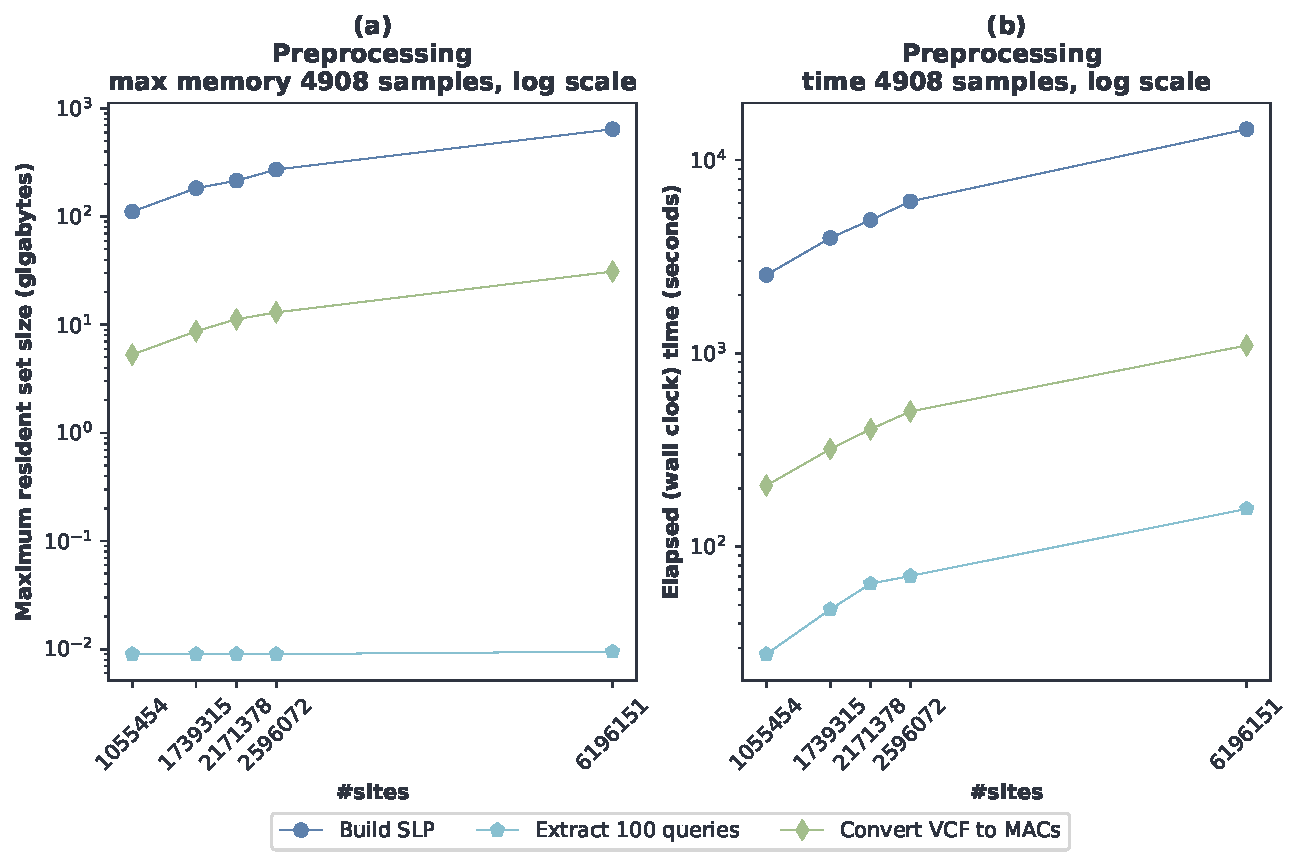
\includegraphics[width=\linewidth]{img/prep_mem_time.pdf}
  \vspace{-5mm}
  \caption{Picchi di memoria (a) e tempo richiesto (b) per le tre fasi di
    preprocessing dell'input per la $\RLPBWT$, in scala logaritmica.}
  \label{fig:prechr}
\end{figure}
\begin{table}
  \centering
  \small
  \caption{Risultati quantitivi dei picchi di memoria (gigabyte) relativi alle
    fasi di 
    preprocessing per l'input delle varianti della $\RLPBWT$.}
  \label{tab:prepmem}
  \vspace{-2mm}
  \begin{tabular}{c||c|c|c}
    \textbf{Chr} & \textbf{Costruzione SLP} & \textbf{Conversione VCF a MaCS}
    & \textbf{Estrazione query}\\
    \hline
    \hline
    \texttt{chr22} & 111 & 5 & 0,0089  \\
    \texttt{chr20} & 183 & 9 & 0,0090 \\
    \texttt{chr18} & 215 & 11 & 0,0090 \\
    \texttt{chr16} & 272 & 13 & 0,0090 \\
    \texttt{chr1} & 644 & 31 & 0,0094 
  \end{tabular}
\end{table}
\begin{table}
  \centering
  \small
  \caption{Risultati quantitivi dei tempi (secondi) relativi alle fasi di
    preprocessing per l'input delle varianti della $\RLPBWT$.}
  \label{tab:preptime}
  \vspace{-2mm}
  \begin{tabular}{c||c|c|c}
    \textbf{Chr} & \textbf{Costruzione SLP} & \textbf{Conversione VCF a MACs}
    & \textbf{Estrazione query}\\
    \hline
    \hline
    \texttt{chr22} & 2542 & 207 & 28 \\
    \texttt{chr20} & 3950 & 320 & 47 \\
    \texttt{chr18} & 4890 & 405 & 64 \\
    \texttt{chr16} & 6104 & 500 & 71 \\
    \texttt{chr1} & 14430 & 1098 & 157
  \end{tabular}
\end{table}
In figura \ref{fig:slpmacschr} si può osservare il vantaggio in termini di
memoria che si ha con l'uso degli $\SLP$, confrontando il peso dei file
MaCS con il peso delle grammatiche compresse. Si segnala che il
peso dei vari file MaCS include anche diversi header. In tabella
\ref{tab:slpmacs} si possono
confrontare quantitativamente tali risultati, notando come usare l'$\,\SLP$
richiede circa l'1\% della memoria necessaria al file non compresso.
\begin{table}
  \centering
  \caption{Dimensioni, in gigabyte, degli $\SLP$ e dei file MaCS
    per i vari pannelli del 1000 Genome Project.}
  \vspace{-2mm}
  \begin{tabular}{c||c|c}
    \textbf{Chr} & \textbf{SLP}
    & \textbf{MaCS} \\
    \hline
    \hline
    \texttt{chr22} & 0,04 & 4,84\\
    \texttt{chr20} & 0,06 & 7,98\\
    \texttt{chr18} & 0,08 & 9,97\\
    \texttt{chr16} & 0,10 & 11,91\\
    \texttt{chr1} & 0,22 & 28,44\\
  \end{tabular}
  \label{tab:slpmacs}
\end{table}
Si noti che, essendo la capacità di compressione di un $\SLP$
direttamente correlata alle ripetizioni presenti nella stringa da comprimere, la
dimensione dell'$\,\SLP$ non è perfettamente proporzionale al numero di siti
dei pannelli in analisi. Per riferimento, comprimere il pannello relativo al
cromosoma 1 con una tecnica standard (GZip), richiede 0,5GB.
\begin{figure}
  \centering
  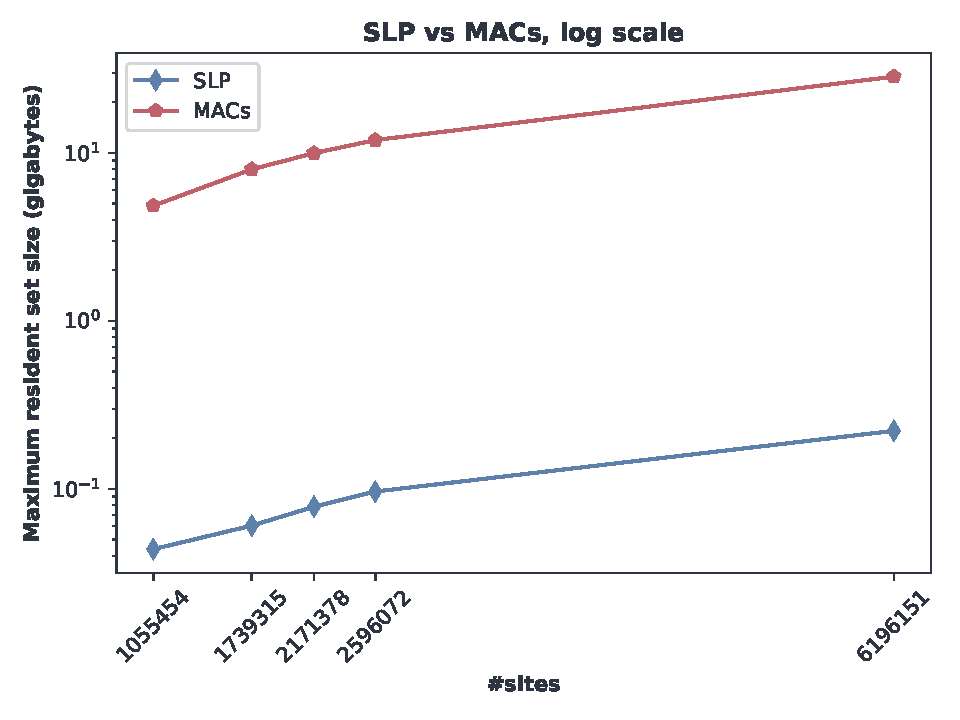
\includegraphics[width=0.7\linewidth]{img/slp_vs_macs_log.pdf}
  \vspace{-5mm}
  \caption{Confronto tra la memoria richiesta dai file MaCS e dagli $\SLP$ per i
    pannelli del 1000 Genome Project, in scala
    logaritmica.} 
  \label{fig:slpmacschr}
\end{figure}
\paragraph{Costruzione della struttura.}
Si analizzano, ora, tempi e picchi di memoria per la costruzione delle
strutture dati. Bisogna ricordare che:
\begin{itemize}
  \item nel caso della $\RLPBWT$, per ognuna delle strutture dati
  composte, questa fase prevede la costruzione e la 
  serializzazione dell'intera struttura dati
  \item nel caso della $\PBWT$, questa fase crea unicamente un file
  compresso ad hoc, contenente le strutture base delle $\PBWT$. A partire
  da tale file, in fase di calcolo degli $\SMEM$, verranno calcolati anche
  tutti gli altri indici necessari al calcolo degli stessi, a seconda
  dell'algoritmo usato 
\end{itemize}
In figura \ref{fig:maketimememchr} (a) vengono visualizzati i picchi di
memoria richiesti mentre in figura \ref{fig:maketimememchr} (b) i tempi di
calcolo delle strutture. Alle tabelle \ref{tab:makemem} e \ref{tab:maketime} si
riportano i risultati quantitativi in termini di gigabyte e secondi.\\ 
Come anticipato, l'implementazione della $\PBWT$ non calcola e memorizza
tutti gli indici 
necessari al calcolo degli $\SMEM$ in fase di costruzione, avendo quindi
una bassissima richiesta di memoria in questa fase.\\
Le strutture dati composte
\texttt{MAP-INT + RLCP} e \texttt{MAP-BV + RLCP}, dovendo 
memorizzare l'intero insieme degli array $\RLCP$, hanno un elevato
consumo di memoria. Pur utilizzando degli intvector compressi, si ha
necessità di salvare $\mathit{NM}$ valori interi. Risulta ovvio notare come, in
termini di costruzione, siano le due strutture che non scalano sul numero
di run 
ad aver maggiori richieste di memoria. Proseguendo nell'analisi si ha che
l'utilizzo della componente 
\texttt{MAP-BV} richiede maggior memoria (approssimativamente tra
il 15\% e il 20\% in più) della componente
\texttt{MAP-INT}, coerentemente con quanto analizzato in Sezione
\ref{sec:comp}. In merito, invece, ai tempi di costruzione delle due 
strutture, si 
segnala come i tempi di calcolo della componente \texttt{MAP-BV} siano superiori
rispetto a quelli della \texttt{MAP-INT} (anche in questo caso
approssimativamente tra il 15\% e il 20\% in più), dovendo
calcolare anche le strutture per le funzioni $\rank$/$\select$ sui bitvector
sparsi. Nel caso della componente 
\texttt{MAP-INT}, invece, l'unica operazione aggiuntiva, rispetto a quelle attese
per una classica popolazione di array di interi, è la fase di compressione degli
stessi. Le analisi effettuate sulle componenti di mapping sono da
ritenersi analoghe a quelle sulle componenti dedicate alle threshold, in
termini d'uso di bitvector sparsi e intvector compressi.
Infine, confrontando le strutture dati in grado
di computare l'array $\MS$, si nota come l'uso della componente \texttt{RA-BV}
comporti, come atteso, una maggior richiesta di memoria, pur limitata dall'uso
dei bitvector, rispetto all'uso della componente
\texttt{RA-SLP}/\texttt{LCE}. Sempre in 
termini di tempi di esecuzione, si ha che la 
componente \texttt{RA-BV} deve essere computata in fase di costruzione delle
strutture, comportando un aumento dei tempi di calcolo (meno del 5\% in
più) rispetto alle strutture basate su
\texttt{RA-SLP}/\texttt{LCE}. Confrontando i tempi di  
tutte le varianti, si ha che tutti gli algoritmi di costruzione sono in tempo
proporzionale a $\mathcal{O}(\mathit{NM})$, ma le varianti della
$\RLPBWT$ includono, in questa fase, anche il calcolo degli indici
utili al calcolo degli $\SMEM$. \\
Si conclude che, parlando di $\RLPBWT$, la
struttura composta \texttt{MAP-INT + LCE + PERM + PHI} risulta essere la meno
costosa in termini di memoria, usando la struttura di mapping tramite
intvector compressi e l'$\,\SLP$ (per le $\LCE$ query).
Anche in termini di tempo risulta essere la soluzione più
vantaggiosa, dovendo costruire meno componenti.\\ 
In generale, si può 
concludere che questo risultato conferma quanto discusso nel capitolo
\ref{metchap}.\\ 
\begin{figure}
  \centering
  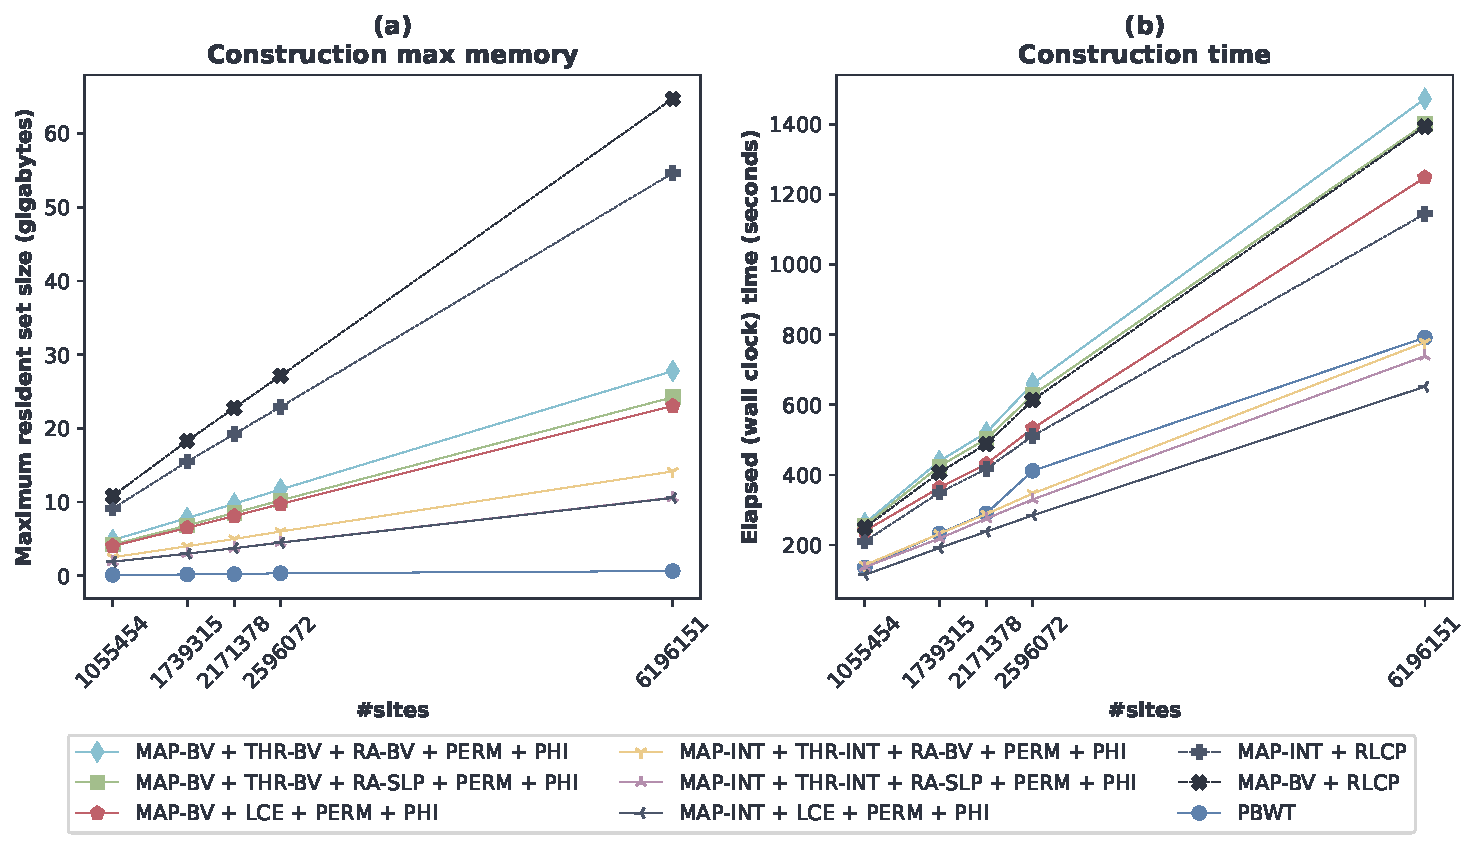
\includegraphics[width=\linewidth]{img/make_time_mem_paper.pdf}
  \vspace{-5mm}
  \caption{Picchi di memoria (a) e tempi di calcolo (b) per la
    costruzione delle varianti della $\RLPBWT$ e per 
    la $\PBWT$.}
  \label{fig:maketimememchr}
\end{figure}
\begin{table}
  \centering
  \caption{Risultati quantitativi dei picchi di memoria (gigabyte) di
    costruzione delle 
    strutture dati.} 
  \label{tab:makemem}
  \footnotesize
  \subcaption*{\footnotesize{Tabella A: risultati relativi alla \textit{PBWT} e
      alle varianti 
      basate su $\RLCP$ per la $\RLPBWT$.}}
  \vspace{+1mm}
  \begin{tabular}{c||c|c|c} 
    \textbf{Chr}
    & \textbf{PBWT}
    & \textbf{\texttt{MAP-INT + RLCP}}
    & \textbf{\texttt{MAP-BV + RLCP}}\\
    \hline
    \hline
    \texttt{chr22} & 0,1 & 9 & 11  \\
    \texttt{chr20} & 0,2 & 15 & 18 \\
    \texttt{chr18} & 0,2 & 19 & 23 \\
    \texttt{chr16} & 0,3 & 23 & 27 \\
    \texttt{chr1} & 0,6 & 55 & 65  \\
  \end{tabular}
  \vspace{+3mm}
  \subcaption*{\footnotesize{Tabella B: risultati relativi alle varianti basate
      su 
      matching statistics e bitvector sparsi per la
      $\RLPBWT$.}}
  \vspace{+1mm}
  \begin{tabular}{c||c|c|c} 
    \textbf{Chr}
    & \textbf{\texttt{MAP/THR-BV + RA-BV $\cdots$}}
    & \textbf{\texttt{MAP/THR-BV + RA-SLP$\cdots$}}
    & \textbf{\texttt{MAP-BV + LCE $\cdots$}}\\
    \hline
    \hline
    \texttt{chr22} & 5 & 4 & 4 \\
    \texttt{chr20} & 8 & 7 & 7 \\
    \texttt{chr18} & 10 & 9 & 8  \\
    \texttt{chr16} & 12 & 10 & 10 \\
    \texttt{chr1} & 28 & 24 & 23 \\
  \end{tabular}
  \vspace{+3mm}
  \subcaption*{\footnotesize{Tabella C: risultati relativi alle varianti basate
      su 
    matching statistics e intvector compressi per la
    $\RLPBWT$.}}
  \vspace{+1mm}
  \begin{tabular}{c||c|c|c} 
    \textbf{Chr}
    & \textbf{\texttt{MAP/THR-INT + RA-BV $\cdots$}}
    & \textbf{\texttt{MAP/THR-INT + RA-SLP $\cdots$}}
    & \textbf{\texttt{MAP-INT + LCE $\cdots$}}\\
    \hline
    \hline
    \texttt{chr22} & 3 & 2 & 2 \\
    \texttt{chr20} & 4 & 3 & 3 \\
    \texttt{chr18} & 5 & 4 & 4 \\
    \texttt{chr16} & 6 & 5 & 5 \\
    \texttt{chr1} & 14 & 12 & 11 
  \end{tabular}
\end{table}
\begin{table}
  \centering
  \caption{Risultati quantitativi dei tempi (secondi) di costruzione delle
    strutture dati.} 
  \label{tab:maketime}
  \footnotesize
  \subcaption*{\footnotesize{Tabella A: risultati relativi alla $\PBWT$ e
      alle varianti 
    basate su $\RLCP$ per la \texttt{\RLPBWT}.}} 
  \begin{tabular}{c||c|c|c} 
    \textbf{Chr}
    & \textbf{PBWT}
    & \textbf{\texttt{MAP-INT + RLCP}}
    & \textbf{\texttt{MAP-BV + RLCP}}\\
    \hline
    \hline
    \texttt{chr22} & 136 & 210 & 250 \\
    \texttt{chr20} & 233 & 349 & 407 \\
    \texttt{chr18} & 290 & 417 & 488 \\
    \texttt{chr16} & 412 & 511 & 613 \\
    \texttt{chr1} & 792 & 1145 & 1393
  \end{tabular}
  \vspace{+3mm}
  \subcaption*{\footnotesize{Tabella B: risultati relativi alle varianti basate
      su 
      matching statistics e bitvector sparsi per la
      $\RLPBWT$.}}
  \vspace{+1mm}
  \begin{tabular}{c||c|c|c} 
    \textbf{Chr}
    & \textbf{\texttt{MAP/THR-BV + RA-BV $\cdots$}}
    & \textbf{\texttt{MAP/THR-BV + RA-SLP $\cdots$}}
    & \textbf{\texttt{MAP-BV + LCE $\cdots$}}\\
    \hline
    \hline
    \texttt{chr22} & 262 & 255 & 240 \\
    \texttt{chr20} & 439 & 424 & 363 \\
    \texttt{chr18} & 521 & 503 & 431 \\
    \texttt{chr16} & 660 & 628 & 533 \\
    \texttt{chr1} & 1472 & 1400 & 1248 
  \end{tabular}
  \vspace{+3mm}
  \subcaption*{\footnotesize{Tabella C: risultati relativi alle varianti basate
      su 
    matching statistics e intvector compressi per la
    $\RLPBWT$.}}
  \vspace{+1mm}
  \begin{tabular}{c||c|c|c} 
    \textbf{Chr}
    & \textbf{\texttt{MAP/THR-INT + RA-BV $\cdots$}}
    & \textbf{\texttt{MAP/THR-INT + RA-SLP $\cdots$}}
    & \textbf{\texttt{MAP-INT + LCE $\cdots$}}\\
    \hline
    \hline
    \texttt{chr22} & 143 & 137 & 115 \\
    \texttt{chr20} & 232 & 219 & 192 \\
    \texttt{chr18} & 288 & 275 & 238 \\
    \texttt{chr16} & 347 & 330 & 285 \\
    \texttt{chr1} & 778 & 739 & 652
  \end{tabular}
\end{table}
Sfruttando i metodi offerti dalla SDSL, è possibile studiare
l'occupazione di memoria delle singole componenti trattate nel capitolo
\ref{metchap}. 
In tabella \ref{tab:comp} e in figura \ref{fig:comp}
si riportano, in megabyte, 
le dimensioni delle varie componenti. Si può,
innanzitutto, apprezzare il vantaggio dell'uso della componente
\texttt{RA-SLP/LCE} rispetto alla 
componente \texttt{RA-BV}, avendo un risparmio di memoria superiore al
90\%. Numericamente tale vantaggio è riportato in tabella
\ref{tab:slppanel}.
\begin{table}
  \centering
  \caption{Vantaggio percentuale dell'uso delle componenti \texttt{RA-SLP/LCE}
    rispetto alla componente \texttt{RA-BV}.}
  \vspace{-2mm}
  \begin{tabular}{c||c|c|c}
    \textbf{Chr} & \textbf{\texttt{RA-SLP/LCE}
                                          (\textit{MB})}
    & \textbf{\texttt{RA-BV} (\textit{MB})} & \textbf{\%}\\
    \hline
    \hline
    \texttt{chr22} & 44 & 628 & 7\\
    \texttt{chr20} & 61 & 1.035 & 6\\
    \texttt{chr18} & 80 & 1.292 & 6\\
    \texttt{chr16} & 98 & 1.544 & 6\\
    \texttt{chr1} & 226 & 3.687 & 6\\
  \end{tabular}
  \label{tab:slppanel}
\end{table}
Si nota, infine, come le componenti \texttt{PERM} e \texttt{PHI} non
presentino particolari criticità dal punto di vista della memoria
richiesta. Terminando l'analisi di tali risultati, senza trattare
nuovamente le componenti per il random access, si ha conferma della
richiesta eccessiva in memoria della componente \texttt{RLCP}.
\begin{figure}
  \centering
  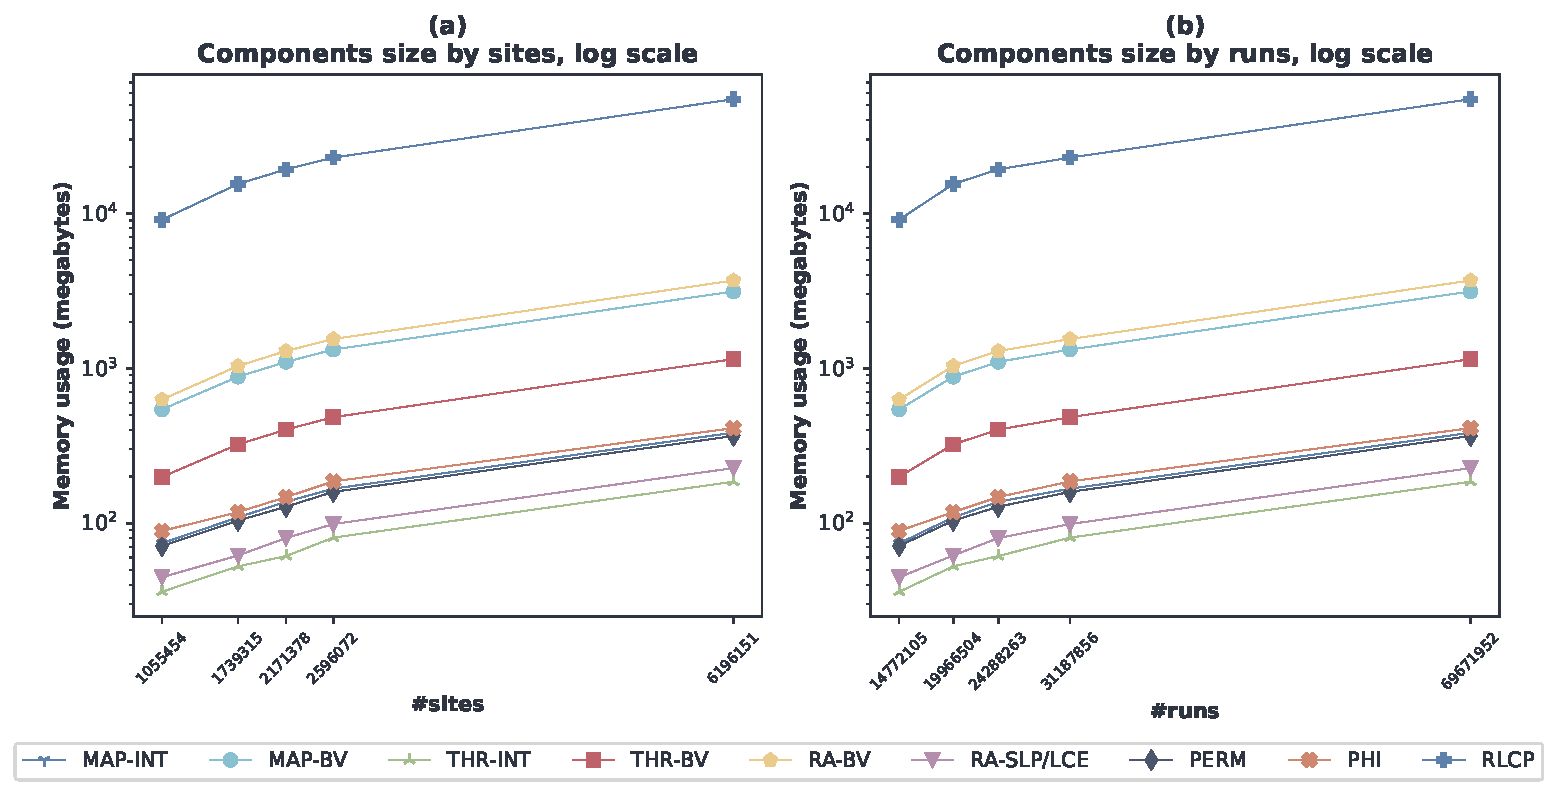
\includegraphics[width=\linewidth]{img/comp_mem.pdf}
  \vspace{-5mm}
  \caption{Memoria occupata dalle singole componenti, avendo sulle ascisse in
    (a) il numero di siti e in (b) il numero di run. }
  \label{fig:comp}
\end{figure}
\begin{table}
  \centering
  \caption{Dimensioni, in megabyte, delle singole componenti per la
    $\RLPBWT$.} 
  \label{tab:comp}
  \subcaption*{\footnotesize{Tabella A: dimensioni delle componenti di
    mapping e threshold usate nelle
    strutture dati per la $\RLPBWT$.}}   
  \begin{tabular}{c||c|c|c|c}
    \textbf{Chr} & \textbf{\texttt{MAP-INT}} & \textbf{\texttt{MAP-BV}}
    & \textbf{\texttt{THR-INT}} & \textbf{\texttt{THR-BV}} \\
    \hline
    \hline
    \texttt{chr22} & 74 & 543 & 36 & 199\\ \hline
    \texttt{chr20} & 109 & 882 & 53 & 322\\ \hline
    \texttt{chr18} & 137 & 1.100 & 61 & 402\\ \hline
    \texttt{chr16} & 167 & 1.320 & 81 & 483\\ \hline
    \texttt{chr1} & 384 & 3.133 & 185 & 1.146
  \end{tabular}
  \vspace{+3mm}
  \subcaption*{\footnotesize{Tabella B: dimensioni delle componenti di
      random access, prefix array sample, struttura $\phi$ e reverse longest
      common prefix.} }
 \vspace{+1mm}
  \begin{tabular}{c||c|c|c|c|c}
    \textbf{Chr} & \textbf{\texttt{RA-BV}} & \textbf{\texttt{RA-SLP/LCE}}
    & \textbf{\texttt{PERM}} & \textbf{\texttt{PHI}} & \textbf{\texttt{RLCP}}\\
    \hline
    \hline
    \texttt{chr22} & 628 & 44 & 71 & 89 & 9.095\\ \hline
    \texttt{chr20} & 1.035 & 62 & 104 & 118 & 15.468 \\ \hline
    \texttt{chr18} & 1.292 & 80 & 128 & 147 & 19.223 \\ \hline
    \texttt{chr16} & 1.545 & 99 & 159 & 186 & 22.888\\ \hline
    \texttt{chr1} & 3.687 & 227 & 366 & 411 & 54.588
  \end{tabular}
\end{table}
\paragraph{Calcolo degli SMEM.}
In seguito si ha la discussione dei risultati ottenuti per il calcolo degli
$\SMEM$.\\ 
In figura \ref{fig:smemtimememchr} (a) si riportano i risultati i termini di
picchi di 
memoria durante la computazione degli $\SMEM$, che sono
consultabili quantitativamente in tabella \ref{tab:exemem}. Come previsto,
l'algoritmo 
\texttt{matchDynamic} della $\PBWT$ ha le migliori prestazioni
in spazio, calcolando dinamicamente i vari indici necessari al computo degli
$\SMEM$ interni. Invece, per quanto riguarda l'algoritmo
5 di Durbin, ovvero l'algoritmo \texttt{matchIndexed}, si confermano le
previsioni 
fatte dall'autore stesso, avendo che la memoria utilizzata è circa
$13\mathit{NM}$ 
byte. Escludendo le strutture \texttt{MAP-INT + RLCP} e \texttt{MAP-BV + RLCP},
si rileva almeno un intero ordine di grandezza in più di memoria rispetto alle
strutture dati composte per la $\RLPBWT$. In esse, la
differenza tra le varie strutture dati che supportano il calcolo 
dell'array $\MS$ è dovuta, a parità di componente per il mapping (e
conseguentemente della componente per le threshold), dall'uso della componente
\texttt{RA-BV} o della componente \texttt{RA-SLP}/\texttt{LCE},
in modo analogo a quanto visto discutendo il peso in memoria
delle singole componenti.\\
% Interessante è notare il rapporto tra la memoria richiesta dalla \textit{RLPBWT}
% con \textit{SLP} e \textit{LCE} e la \textit{PBWT Indexed}:
% \begin{table}[H]
%   \centering
%   \footnotesize
%   \begin{tabular}{c|c|c|c|c}
%     \textbf{\#Samples} & \textbf{\#Siti}
%     & \textbf{RLPBWT SLP-LCE (\textit{kb})}
%     & \textbf{PBWT Indexed (\textit{kb})} & \textbf{\%}\\
%     \hline
%     4908 & 1055454 & 3058088 & 65975520 & 4.64\\
%     4908 & 1739315 & 4961664 & 108713424 & 4.56\\
%     4908 & 2171378 & 6190684 & 135726084 & 4.56\\
%     4908 & 2596072 & 7430300 & 162257008 & 4.58\\
%     4908 & 6196151 & 17635700 & 387252160 & 4.55
%   \end{tabular}
% \end{table}
% Anche in questo caso le percentuali risultano leggermente peggiori rispetto ai
% pannelli simulati, pur restando risultati molto interessanti.
In figura \ref{fig:smemtimememchr} (b) si riportano, invece, i risultati i
termini di tempo di calcolo,
consultabili numericamente in tabella \ref{tab:exetime}. Anche in questo caso,
l'algoritmo 
\texttt{matchDynamic} risulta essere il più performante, in quanto studia
contemporaneamente l'intero pannello di query. Parlando di $\RLPBWT$,  la
struttura \texttt{MAP-INT + THR-INT + RA-SLP + PERM + PHI} e la 
struttura 
\texttt{MAP-BV + THR-BV + RA-SLP + PERM + PHI}, a causa delle
frequenti operazioni di random access con la componente
\texttt{RA-SLP} (sia per il calcolo delle lunghezze delle 
matching statistics che per la fase di disambiguazione), richiedono più tempo
di tutte le altre varianti, soprattutto se si pensa alle corrispondenti
varianti con componente \texttt{RA-BV}. L'uso della componente \texttt{RA-SLP}
comporta, infatti, circa 20 volte i tempi di calcolo, rispetto all'uso della
componente \texttt{RA-BV}, nelle strutture composte
basate su bitvector sparsi e di circa 45 volte in quelle basate su intvector
compressi. La struttura 
\texttt{MAP-INT + LCE + 
  PERM + PHI} e la struttura 
\texttt{MAP-BV + LCE + PERM + PHI} risultano essere, al massimo,
il doppio più lente rispetto all'algoritmo \texttt{matchIndexed}, con una
differenze che diventa quasi trascurabile all'aumentare delle dimensioni del
pannello. Questo è un 
risultato molto interessante, considerando la memoria necessaria
per il calcolo degli $\SMEM$ delle varie implementazioni.\\
Confrontando l'uso delle $\LCE$ query con quello della componente
\texttt{RA-BV}, si hanno, invece, tempi triplicati nel caso d'uso di componenti
per mapping e 
threshold con bitvector sparsi. In caso di utilizzo degli intvector compressi,
si 
hanno circa sette volte i tempi di 
computazione. A priori delle componenti per mapping e
threshold, l'uso della componente \texttt{RA-SLP} comporta circa sei
volte il tempo che si ha con le $\LCE$ query. Queste ultime analisi comportano
che l'uso del random access su $\SLP$ è la peggior soluzione in
ottica di calcolo delle matching statistics.\\
Concludendo, si può notare come la struttura composta
\texttt{MAP-INT + THR-INT + RA-BV + PERM + PHI}, tra quelle per la
$\RLPBWT$, risulta essere la migliore in termini di tempi di calcolo
mentre la struttura composta \texttt{MAP-INT + LCE + PERM + PHI} è la
migliore in termini di memoria richiesta. Questo risultato è coerente con quanto
analizzato nel Capitolo \ref{metchap}. Notando come quest'ultima sia quasi 10
volte più lenta della soluzione con \texttt{THR-INT} e \texttt{RA-BV}, si può
inferire come la scelta della miglior soluzione per la 
$\RLPBWT$ debba ricadere sulla \texttt{MAP-INT + THR-INT + RA-BV + PERM +
  PHI}, salvo situazioni in cui il risparmio di memoria sia
fondamentale in fase di analisi dati. 
\begin{figure}
  \centering
  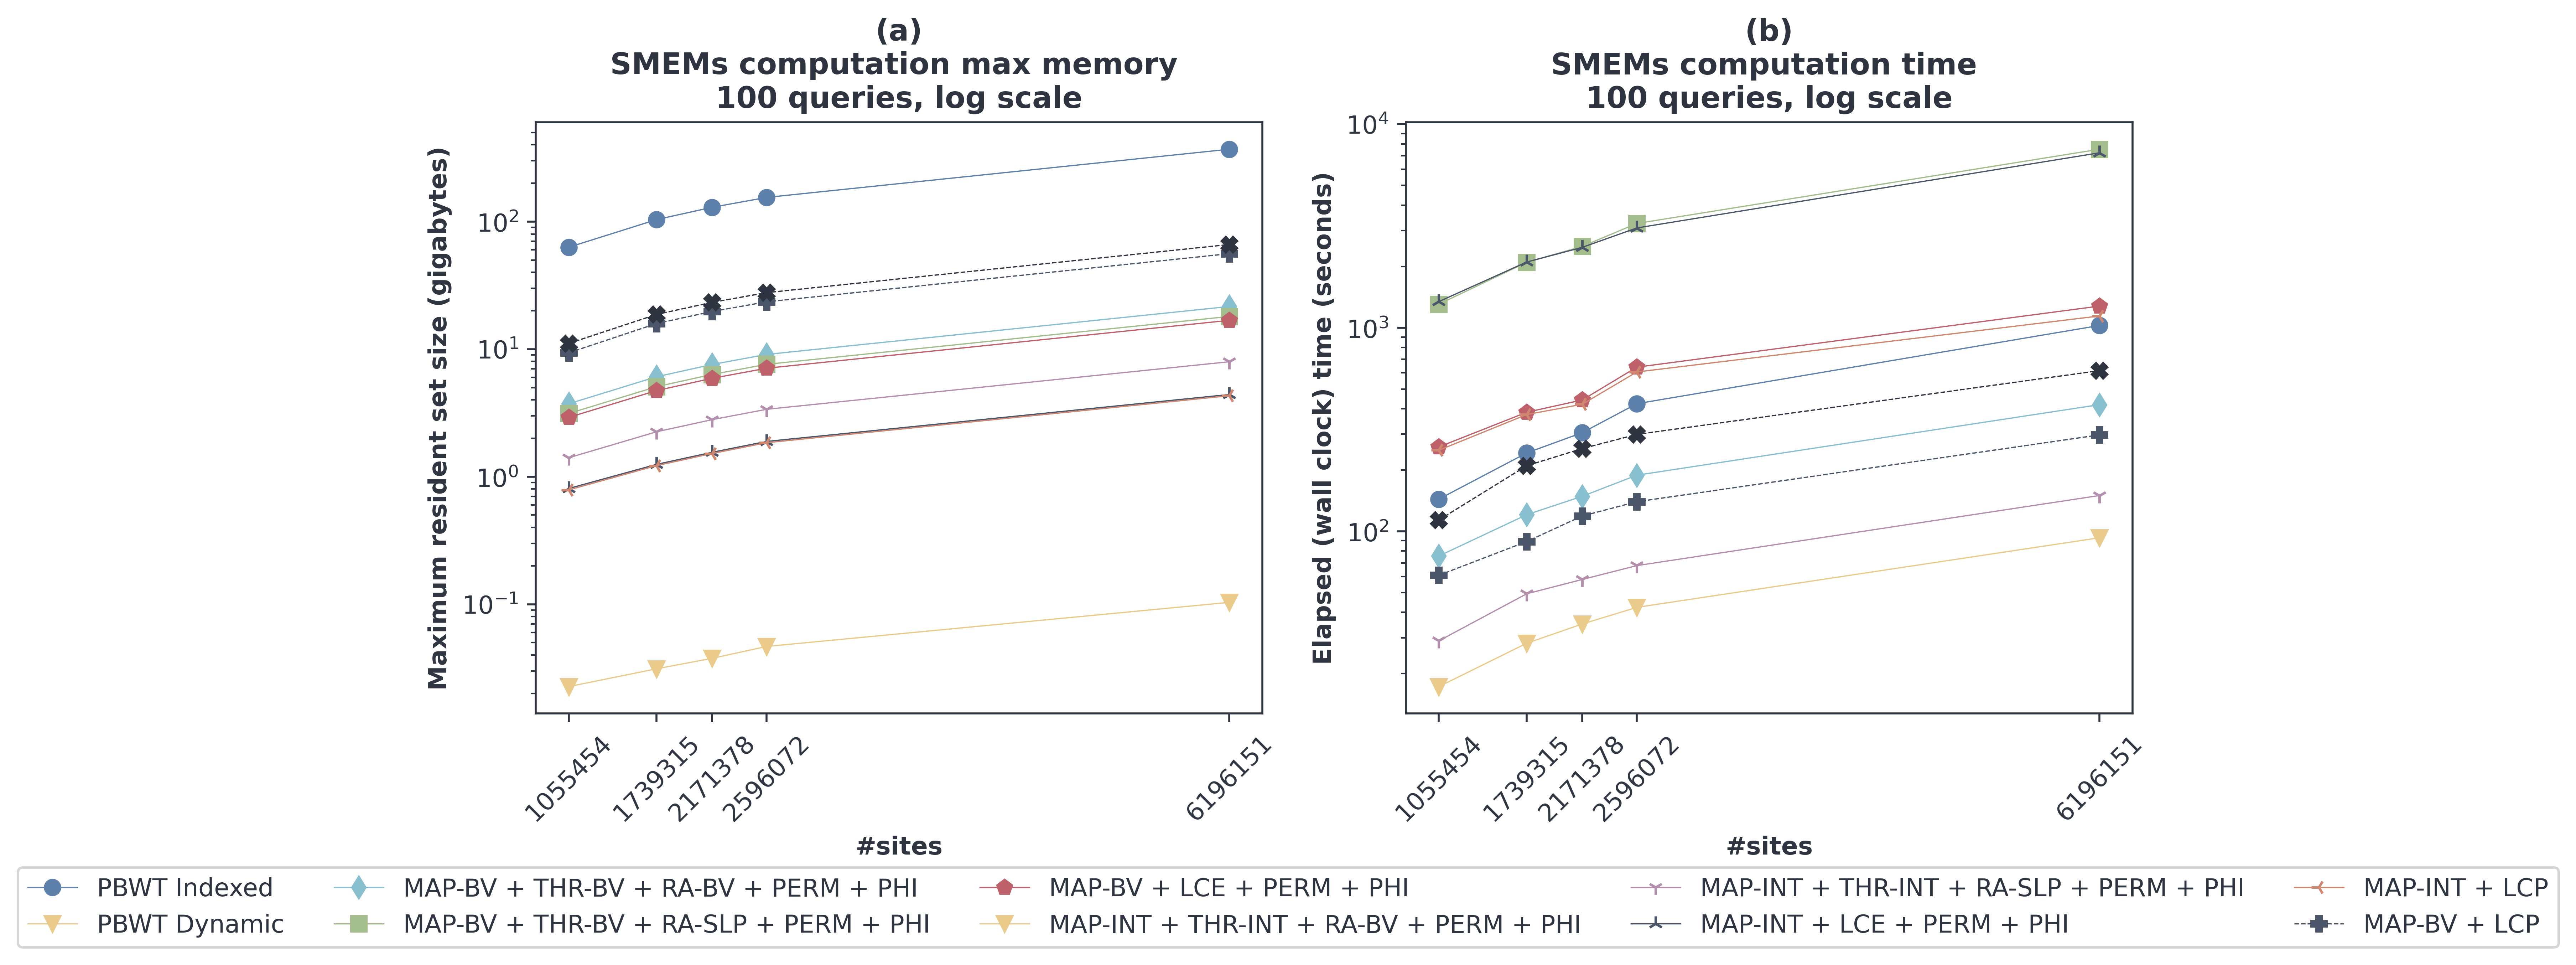
\includegraphics[width=\linewidth]{img/exe_time_mem_paper}
  \vspace{-5mm}
  \caption{Picchi di memoria (a) e tempi di esecuzione (b) per il calcolo degli
    $\SMEM$.}
  \label{fig:smemtimememchr}
\end{figure}
\begin{table}
  \centering
  \caption{Risultati quantitativi dei picchi di memoria (gigabyte)
    di calcolo degli $\SMEM$.} 
  \label{tab:exemem}
  \footnotesize
  \subcaption*{\footnotesize{Tabella A: risultati relativi alla $\PBWT$ e
      alle varianti 
      basate su $\RLCP$ per la $\RLPBWT$.}}
  \vspace{-2mm}
  \begin{tabular}{c||c|c|c|c} 
    \textbf{Chr}
    & \textbf{\texttt{matchIndexed}}
    & \textbf{\texttt{matchDynamic}}
    & \textbf{\texttt{MAP-INT + RLCP}}
    & \textbf{\texttt{MAP-BV + RLCP}}\\
    \hline
    \hline
    \texttt{chr22} & 63 & 0,02 & 9 & 11 \\
    \texttt{chr20} & 104 & 0,03 & 16 & 19 \\
    \texttt{chr18} & 129 & 0,04 & 20 & 23 \\
    \texttt{chr16} & 155 & 0,05 & 24 & 28 \\
    \texttt{chr1} & 369 & 0,10 & 56 & 66 
  \end{tabular}
  \vspace{+3mm}
  \subcaption*{\footnotesize{Tabella B: risultati relativi alle varianti basate
      su 
      matching statistics e bitvector sparsi per la
      $\RLPBWT$.}}
  \vspace{+1mm}
  \begin{tabular}{c||c|c|c} 
    \textbf{Chr}
    & \textbf{\texttt{MAP/THR-BV + RA-BV $\cdots$}}
    & \textbf{\texttt{MAP/THR-BV + RA-SLP $\cdots$}}
    & \textbf{\texttt{MAP-BV + LCE $\cdots$}}\\
    \hline
    \hline
    \texttt{chr22} & 4 & 3 & 3  \\
    \texttt{chr20} & 6 & 5 & 5 \\
    \texttt{chr18} & 8 & 6 & 6 \\
    \texttt{chr16} & 9 & 8 & 7 \\
    \texttt{chr1} & 22 & 18 & 17 
  \end{tabular}
  \vspace{+3mm}
  \subcaption*{\footnotesize{Tabella C: risultati relativi alle varianti basate
      su 
    matching statistics e intvector compressi per la
    $\RLPBWT$.}}
  \vspace{+1mm}
  \begin{tabular}{c||c|c|c} 
    \textbf{Chr}
    & \textbf{\texttt{MAP/THR-INT + RA-BV $\cdots$}}
    & \textbf{\texttt{MAP/THR-INT + RA-SLP $\cdots$}}
    & \textbf{\texttt{MAP-INT + LCE $\cdots$}}\\
    \hline
    \hline
    \texttt{chr22} & 1,4 & 0,8 & 0,8 \\
    \texttt{chr20} & 2,2 & 1,2 & 1,2 \\
    \texttt{chr18} & 2,8 & 1,6 & 1,5 \\
    \texttt{chr16} & 3,4 & 1,9 & 1,8 \\
    \texttt{chr1} & 8,0 & 4,4 & 4,3                                           
  \end{tabular}
\end{table}
\begin{table}
  \centering
  \caption{Risultati quantitativi dei tempi (secondi) di calcolo degli
    $\SMEM$.}  
  \label{tab:exetime}
  \footnotesize
  \subcaption*{\footnotesize{Tabella A: risultati relativi alla $\PBWT$ e
      alle varianti 
      basate su $\RLCP$ per la $\RLPBWT$.}}
  \vspace{-2mm}
  \begin{tabular}{c||c|c|c|c} 
    \textbf{Chr}
    & \textbf{\texttt{matchIndexed}}
    & \textbf{\texttt{matchDynamic}}
    & \textbf{\texttt{MAP-INT + RLCP}}
    & \textbf{\texttt{MAP-BV + RLCP}}\\
    \hline
    \hline
    \texttt{chr22} & 144 & 17 & 61 & 114 \\
    \texttt{chr20} & 243 & 28 & 89 & 210 \\
    \texttt{chr18} & 305 & 35 & 119 & 255 \\
    \texttt{chr16} & 424 & 42 & 140 & 299 \\
    \texttt{chr1} & 1026 & 93 & 298 & 616
  \end{tabular}
  \vspace{+3mm}
  \subcaption*{\footnotesize{Tabella B: risultati relativi alle varianti basate
      su 
      matching statistics e bitvector sparsi per la
      $\RLPBWT$.}}
  \vspace{+1mm}
  \begin{tabular}{c||c|c|c} 
    \textbf{Chr}
    & \textbf{\texttt{MAP/THR-BV + RA-BV $\cdots$}}
    & \textbf{\texttt{MAP/THR-BV + RA-SLP $\cdots$}}
    & \textbf{\texttt{MAP-BV + LCE $\cdots$}}\\
    \hline
    \hline
    \texttt{chr22} & 76 & 1305 & 260 \\
    \texttt{chr20} & 121 & 2097 & 385  \\
    \texttt{chr18} & 149 & 2509 & 442  \\
    \texttt{chr16} & 189 & 3252 & 640 \\
    \texttt{chr1} & 419 & 7531 & 1278 
  \end{tabular}
  \vspace{+3mm}
  \subcaption*{\footnotesize{Tabella C: risultati relativi alle varianti basate
      su 
    matching statistics e intvector compressi per la
    $\RLPBWT$.}}
  \vspace{+1mm}
  \begin{tabular}{c||c|c|c} 
    \textbf{Chr}
    & \textbf{\texttt{MAP/THR-INT + RA-BV $\cdots$}}
    & \textbf{\texttt{MAP/THR-INT + RA-SLP $\cdots$}}
    & \textbf{\texttt{MAP-INT + LCE $\cdots$}}\\
    \hline
    \hline
    \texttt{chr22} & 29 & 1344 & 250 \\
    \texttt{chr20} & 49 & 2103 & 375 \\
    \texttt{chr18} & 58 & 2483 & 421 \\
    \texttt{chr16} & 68 & 3092 & 606 \\
    \texttt{chr1} & 150 & 7234 & 1142

  \end{tabular}
\end{table}
\subsection{Tempo di una singola query}
Infine, per completare lo studio delle prestazioni dal punto di vista del tempo
macchina, si è deciso di 
isolare il calcolo degli $\SMEM$ per ogni singola query, valutando media e
deviazione standard dell'esecuzione su 100 query. A tal fine, la misurazione è
stata 
effettuata sfruttando la libreria \texttt{time.h} presente nello standard del
linguaggio C, per avere le medesime istruzioni relative alle misurazioni sia con
la $\PBWT$ 
che con la $\RLPBWT$. La misurazione è stata fatta considerando unicamente le
istruzioni atte a cercare gli $\SMEM$, 
escludendo quelle per il computo degli indici o del caricamento delle strutture
dati.
Si segnala che, nel caso dell'algoritmo \texttt{matchDynamic}, non si è
potuto, per natura stessa dell'algoritmo, isolare l'aggiornamento degli indici
all'avanzamento alla colonna successiva. Resta esclusa, in ogni caso, la
costruzione della struttura base della $\PBWT$.\\
Tale risultato è visualizzabile in figura
\ref{fig:smemsinglechr}, dove si è deciso di escludere le strutture
\texttt{MAP-INT + RLCP} e \texttt{MAP-BV + RLCP} in quanto non in grado di
computare quali righe presentino un certo $\SMEM$. I risultati
quantitativi sono consultabili in tabella \ref{tab:exetimesingle}. Anche in
questo caso, 
si conferma molto di quanto ipotizzato e discusso nel Capitolo
\ref{metchap} e nella sezione precedente. Nel caso dell'algoritmo
\texttt{matchIndexed}, non misurando le istruzioni per computare 
tutti gli array necessari, si hanno tempi di calcolo degli $\SMEM$ migliori di
quanto visto sull'esecuzione completa. Caso a parte
è dato dall'algoritmo \texttt{matchDynamic}, che risulta avere le performance
peggiori, impiegando fino a cento volte il tempo dell'algoritmo 5 di
Durbin, ovvero l'algoritmo \texttt{matchIndexed}. Infatti, per natura stessa
dell'algoritmo,  
le operazioni sono studiate al fine di essere ottimizzate per pannelli di query
e non per una query singola, avendo molte
operazioni che potrebbero essere ottimizzate analizzando una singola
query. Sperimentalmente, si è
osservato che una query o un centinaio di query presentano all'incirca i
medesimi tempi di calcolo. Infatti, prendendo ad esempio il cromosoma 1, si ha
che tale 
algoritmo impiega 93s per il calcolo con 100 query e una media di circa 88s (con
una deviazione standard di ben 7s) per
una singola query. Per quanto riguarda la $\RLPBWT$, con l'uso della
componente \texttt{RA-SLP}, si rilevano gli stessi problemi relativi al random
access, precedentemente descritti. Questi problemi sono risolti con l'uso della
componente \texttt{RA-BV}. Inoltre, a parità di componenti per il mapping (e
conseguenti componenti per le threshold), l'uso della componente \texttt{LCE}
risulta più lento dell'uso della componente \texttt{RA-BV}, a causa dei costi di
calcolo delle $\LCE$ query stesse. Tutti questi sono risultati coerenti
con quanto visto nel caso di 100 query, anche in termini di migliori strutture
composte parlando di $\RLPBWT$. Si segnala che, oltre al fatto che non
sono qui misurate le tempistiche di caricamento delle strutture, le acquisizioni
dei dati 
per la singola query sono state ottenute in un momento diverso da quelle per 100
query, avendo, di conseguenza, una correlazione non perfetta tra i risultati
quantitativi delle due fasi della sperimentazione.
\begin{figure}
  \centering
  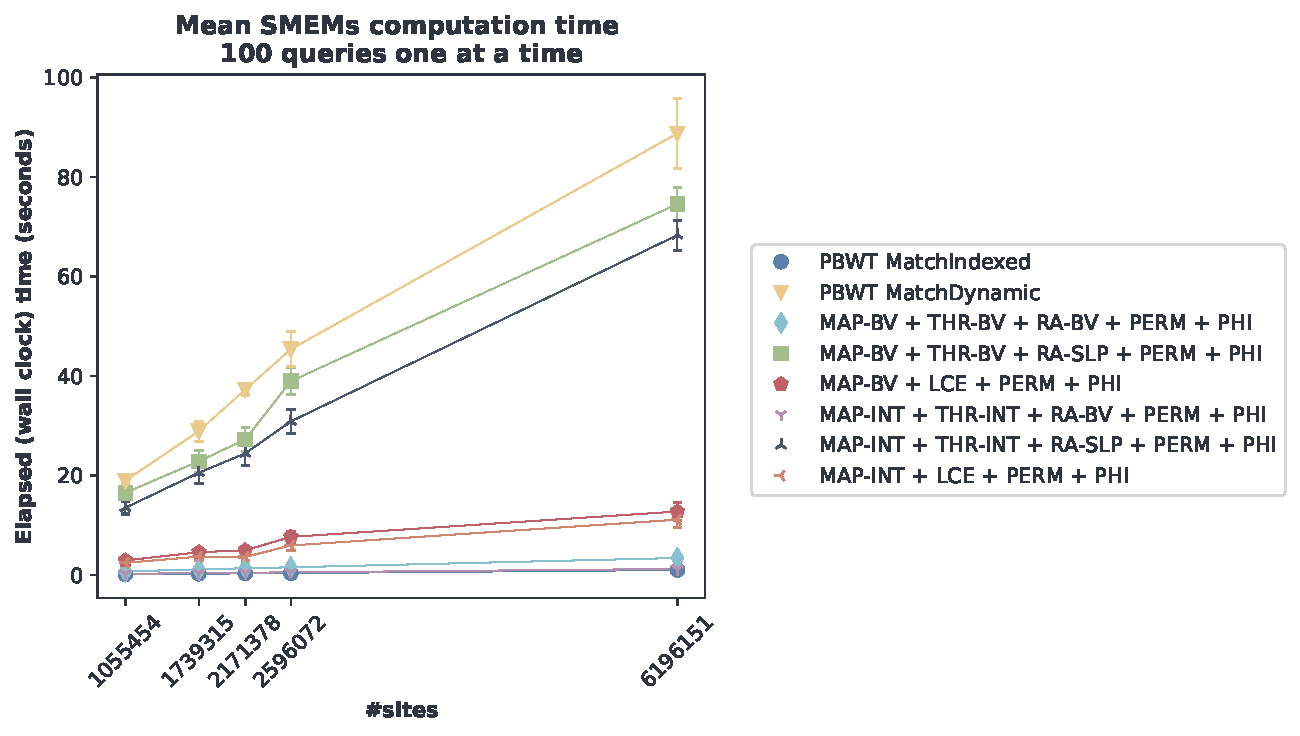
\includegraphics[width=\textwidth]{img/exe_time_single_paper.pdf}
  \vspace{-5mm}
  \caption{Tempo medio di esecuzione del calcolo degli $\SMEM$ per una singola
    query. Le
    barre d'errore rappresentano la deviazione standard.}
  \label{fig:smemsinglechr}
\end{figure}

\begin{table}
  \centering
  \caption{Risultati quantitativi dei tempi (secondi) di calcolo degli
    $\SMEM$ su singola query. I risultati sono nella forma ``media $\pm$
    deviazione standard''.}  
  \label{tab:exetimesingle}
  \footnotesize
  \subcaption*{\footnotesize{Tabella A: risultati relativi alla $\PBWT$.}}
  \vspace{-2mm}
  \begin{tabular}{c||c|c} 
    \textbf{Chr}
    & \textbf{\texttt{matchIndexed}}
    & \textbf{\texttt{matchDynamic}}\\
    \hline
    \hline
    \texttt{chr22} & 0,15 $\pm$ 0,01 & 18,94 $\pm$ 0,58 \\
    \texttt{chr20} & 0,25 $\pm$ 0,01 & 28,90 $\pm$ 1,99 \\
    \texttt{chr18} & 0,33 $\pm$ 0,02 & 37,24 $\pm$ 1,08  \\
    \texttt{chr16} & 0,38 $\pm$ 0,01 & 45,37 $\pm$ 3,49 \\
    \texttt{chr1} & 1,01 $\pm$ 0,10 & 88,73 $\pm$ 7,08
  \end{tabular}
  \vspace{+3mm}
  \subcaption*{\footnotesize{Tabella B: risultati relativi alle varianti basate
      su 
      matching statistics e bitvector sparsi per la
      $\RLPBWT$.}}
  \vspace{+1mm}
  \begin{tabular}{c||c|c|c} 
    \textbf{Chr}
    & \textbf{\texttt{MAP/THR-BV + RA-BV $\cdots$}}
    & \textbf{\texttt{MAP/THR-BV + RA-SLP $\cdots$}}
    & \textbf{\texttt{MAP-BV + LCE $\cdots$}}\\
    \hline
    \hline
    \texttt{chr22} & 0,75 $\pm$ 0,28 & 16,51 $\pm$ 1,34 & 2,92 $\pm$ 0,55\\
    \texttt{chr20} & 1,08 $\pm$ 0,05 & 22,85 $\pm$ 2,21 & 4,57 $\pm$ 0,82\\
    \texttt{chr18} & 1,36 $\pm$ 0,05 & 27,23 $\pm$ 2,50 & 4,96 $\pm$ 0,74 \\
    \texttt{chr16} & 1,54 $\pm$ 0,05 & 38,93 $\pm$ 2,70 & 7,65 $\pm$ 1,14 \\
    \texttt{chr1} & 3,41 $\pm$ 0,07 & 74,54 $\pm$ 3,40 & 12,75 $\pm$ 1,82 
  \end{tabular}
  \vspace{+3mm}
  \subcaption*{\footnotesize{Tabella C: risultati relativi alle varianti basate
      su 
    matching statistics e intvector compressi per la
    $\RLPBWT$.}}
  \vspace{+1mm}
  \begin{tabular}{c||c|c|c} 
    \textbf{Chr}
    & \textbf{\texttt{MAP/THR-INT + RA-BV $\cdots$}}
    & \textbf{\texttt{MAP/THR-INT + RA-SLP $\cdots$}}
    & \textbf{\texttt{MAP-INT + LCE $\cdots$}}\\
    \hline
    \hline
    \texttt{chr22} & 0,24 $\pm$ 0,02 & 13,52 $\pm$ 1,26 & 2,44 $\pm$ 0,54 \\
    \texttt{chr20} & 0,37 $\pm$ 0,03 & 20,55 $\pm$ 2,16 & 3,68 $\pm$ 0,74 \\
    \texttt{chr18} & 0,45 $\pm$ 0,03 & 24,43 $\pm$ 2,38 & 3,86 $\pm$ 0,70 \\
    \texttt{chr16} & 0,54 $\pm$ 0,03 & 30,86 $\pm$ 2,35 & 5,93 $\pm$ 1,01 \\
    \texttt{chr1} & 1,21 $\pm$ 0,06 & 68,22 $\pm$ 3,02 & 11,12 $\pm$ 1,52

  \end{tabular}
\end{table}

% LocalWords:  sottostrutture gigabyte
